\chapter{Detection of rotational spherical aggregate rotational dynamics}
\textit{\textbf{Add overview here}} \\
\label{chapter:simulated_detection}

\section{Overview}
In this chapter we go about defining an optical fibre detection 
system from a mathematical perspective. Before demonstrating how 
it can be used to instantaneously predict orientational information 
on a trapped particle. We then consider common factors of error in the 
characterisation process, such as signal error, and incorrect particle 
sizing. Both of which have a significant impact on the performance 
of the model, but by utilising Bayesian inference, and time averaging 
we can better refine our prediction to a satisfactory degree.   

\section{Introduction}
As outlined in the end of Chapter 3, one of the difficulties 
in characterising interactions with asymmetric objects is 
the coupled motion between translation and rotation. In order
to characterise the optical trap a position detection system 
such as a lateral effect photodiode or a quadrant photo diode
(see fig.\ref{fig:position_detectors}). Typically, a position 
detection system assumes that there exists a linear relationship 
between the a particle's displacement and the detected signal.
However, this is not always the case as demonstrated in chapter
4; as dimer's demonstrate non-harmonic trapping beyond a certain 
displacement. In addition, the rotational effects of the trapped
dimer become a more significant factor when characterising the 
trap strength. This can have unintended effects when it comes to
areas of research that require a precise understanding of the 
hydrodynamic behaviour of particles. As such there has been a 
concerted effort to either eliminate rotational motion, or describe
how the rotational behaviour influences the trajectory reported 
by the position detector. 

In this chapter we build upon the work of \cite{BarZiv1997} to 
determine the instantaneous orientation of the aggregate. Using 
static light scattering we can map the outputted signal from a 
optically trapped dimer to its expected orientation in real time. 
Thus allowing us to estimate the optical torque being applied to 
the dimer by the trapping beam. As demonstrated in chapter 3, 
the influence of a circularly polarised beam can result in 
gyroscopic precession for specifically sized dimers. 


\section{Monitoring Stochastic rotational motion using static 
		light scattering}
Part of the optical fibre arrangement borrows code from the 
optical tweezer simulations discussed in Chapter 2 and 4. 
Rather than repeat the simulation details we will instead 
only focus on the specifics of the optical fibre scattering.

\subsection{Coordinate System}
Consider a particle (either a sphere or dimer) trapped by
a Gaussian beam, with its focal point being set at [0,0,0]. 
At the same time an optical fibre directs a plane wave that 
is incident on the trapped particle scattering light in all 
directions. The probe beam is assumed to be x-polarised and 
propagating in the +z direction, this is a $90^{\circ}$ 
rotation from the previous simulations (see fig\emph{X.X}). 

\subsection{Dimer}
The dimer is defined by two spheres with refractive indices
of 1.59 and suspended in water ($n_{med} = 1.33$). \textit{MSTM}
requires a target origin for setting the scattering expansion, 
there is no agreed upon solution for where the target origin 
should be relative to the sphere positions. In chapter 4 we showed
that altering the target origin would drastically alter the 
tmatrix produced. We choose (somewhat arbitrary) to use 
the dimer's centre of diffusion which is located $\zeta a_I$ from 
the centre of the larger sphere. For a discussion see \emph{X.X}.

\subsection{Scattering and Detection}
Each detector is placed some distance $\bf r$ from the origin, 
detector positions are defined by angles $\theta$ \& $\phi$. With 
$\theta=\phi=0$ being directly in front of the probe beam. The 
position of each detector is given by:
\begin{align}
	\begin{pmatrix}
		x_{fiber} \\ y_{fiber} \\ z_{fiber}
	\end{pmatrix} = 
	\begin{pmatrix}
		rcos(\phi)sin(\theta) \\ rsin(\phi)sin(\theta) \\ rcos(\theta)]
	\end{pmatrix}
\end{align}
Where r is the distance between the detector and the target origin. 
In an ideal situation the surface of the detector is oriented towards 
the target origin perfectly. Pixels can be thought of as points lying 
on the surface of the detector, each point has its own position in real
space. Using \textit{mstm} we can find the components of the scattering 
matrix at each point and compute the intensity of the electric field via:

\begin{align}
	\begin{pmatrix}
		I_s \\ Q_s \\ U_s \\ V_s
	\end{pmatrix} = 
	\begin{pmatrix}
		S_{11} & S_{12} & S_{13} & S_{14} \\
		S_{21} & S_{22} & S_{23} & S_{24} \\
		S_{31} & S_{32} & S_{33} & S_{34} \\
		S_{41} & S_{42} & S_{43} & S_{44} \\
	\end{pmatrix}
	\begin{pmatrix}
		I_i \\ Q_i \\ U_i \\ V_i
	\end{pmatrix}
\end{align}
Where:
\begin{align}
	I_s &= E_{x,\ scat}^2+E_{y,\ scat}^2  \label{eq:intensity} 
	\\
	\rightarrow I_s &= S_{11}I_i+S_{12}Q_i+S_{13}U_i+S_{14}V_i
\end{align}

By computing the scattering at each point on the detectors surface 
we can compute the average scattering over the detector. From a
experimental perspective the distance from the particle to the 
detectors must be considered. The near field scattering can be 
computed with relative ease using \textit{mstm} as shown in 
\begin{figure}[h!]
	\centering
	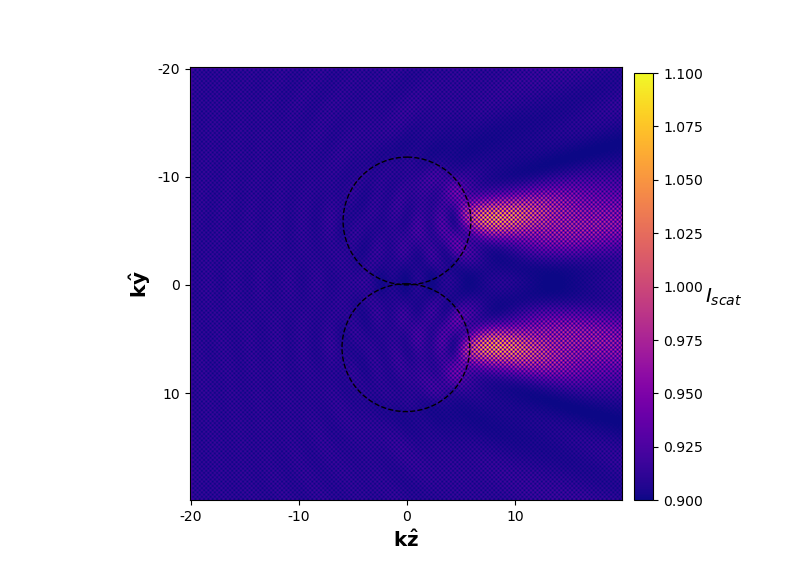
\includegraphics[width=\linewidth]{near_field_intensity_side_profile.png}
	\caption{Intensity distribution (as defined by \eqref{eq:intensity}) 
		from a symmetric dimer when irradiated by the probe beam 
		propagating in the $k\hat{z}$ direction (viewed in the 
		z-y plane). Axis are given in dimensionless units of 
		$k\hat{z}$ and $k\hat{y}$.}
	\label{fig:nf_scattering}
\end{figure}

While \textit{mstm} does provide the amplitude matrix it is not
scaled to account for distance from the target to the detector.
We amend this by simply scaling according to the inverse square 
law. As the detector is moved further from the target the 
intensity distribution across the entire detector will decrease
substantially. Because of the fall off it is more computationally
efficient to instead consider only the central pixel of the 
detector rather than across the entire surface. If we consider 
the difference between the average intensity and the intensity 
of the central point we can see that after not even $20 \mu$ 
away from the target particle the average intensity across the 
surface is within $0.1\%$ of the central pixel. 
\begin{figure}[h!]
	\centering
	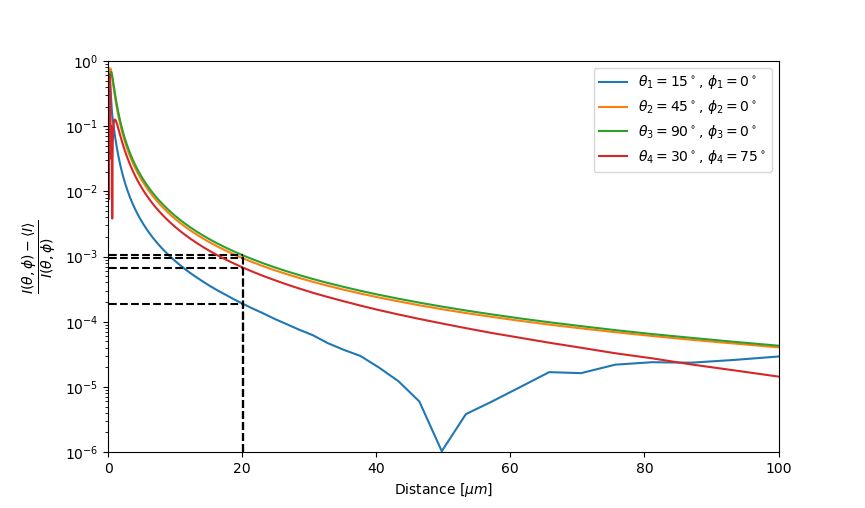
\includegraphics[width=\linewidth]{fall_off_with_distance.png}
	\caption{Normalised difference between the central pixel intensity
	$I(\theta, \phi)$ and the average pixel intensity over the surface
	of the optical fibre $\langle I \rangle$ as a function of distance.
	4 different optical detectors were tested (spherical coordinates 
	are given in the legend). While the choice of coordinates is 
	arbitrary they all demonstrate the same exponential decay. Dashed
	lines indicate the difference after $20\mu m$ from the trap focus,
	in most practical cases getting an optical fibre any closer would
	disrupt the trap stability.}
\end{figure}

Given the trapping beam's beam waist is approximately $0.54 \mu m$,
a optical fibre would need to be a minimum of $150 \mu m$ from the 
trap centre in order to prevent noise from the trapping laser itself.
At such a distance the variation in the signal is so small that it is 
easier to evaluate the intensity at the centre of the detector instead
of across the entire surface. This is how the instantaneous orientation
is predicted later on in the chapter.

\section{Interpretation of scattering data into orientation estimates}
We now discuss the methodology for computing the instantaneous 
orientation of an optically trapped particle based on scattering
detected by a finite grouping of optical fibres. 

Consider a dimer in the optical trap (Fig.~\ref{fig:dimer}a), 
we can define at any point in time a unit vector $\hat{s}$ 
pointing from the centre of the larger sphere to the centre 
of the smaller sphere. A plane wave probe beam incident, 
is incident on the dimer, generating a scattering pattern
dependent on the dimer's orientation $I(\hat{\bf s}, 
\theta, \phi)$ which is computed using \textit{mstm} 
\cite{I.Mishchenko1996}. To represent the experimental set 
up consisting of a set of optical fibres recording scattered 
light, we choose four sets of spherical angles [$(\theta_1,\ 
\phi_1), \ (\theta_2,\ \phi_2), \ (\theta_3, \ \phi_3), \ 
(\theta_4,\ \phi_4)$] and record the calculated intensity at 
each angle $I(\hat{s},\ \theta_k,\ \phi_k)$. 
\begin{figure}[h!]
	\centering
	\begin{subfigure}{0.49\textwidth}
		\subcaption{}
		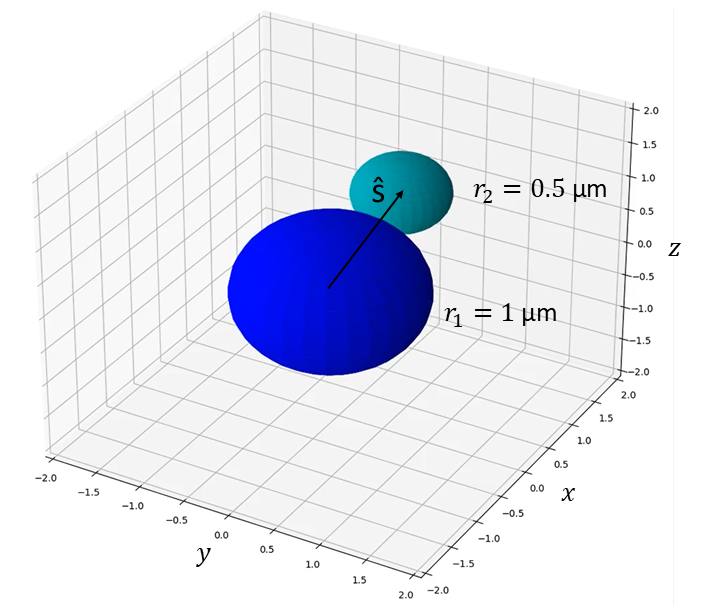
\includegraphics[width=\textwidth]{fig2a.png}
	\end{subfigure}
	\begin{subfigure}{0.49\textwidth}
		\subcaption{}
		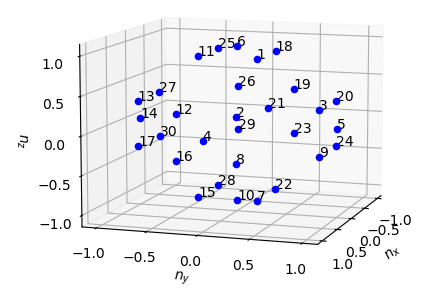
\includegraphics[width=\textwidth]{fig2b.png}
	\end{subfigure}
	\caption{(a)Example dimer in orientation $\hat{\bf s}$, (b) 30 Reference orientations represented by vectors pointing from [0,0,0] to each point}
	\label{fig:dimer}
\end{figure}

Our goal is to determine the orientation of the trapped dimer 
based on the measured intensity $I(\hat{n}, \ \theta_k,\ \phi_k)$. 
Rather than aim an exact estimate of the dimer's orientation, 
for the purposes of interpretation of the scattering and 
optimisation of the measurement setup it is more convenient 
to discretize the possible orientation space into a number 
of possible reference orientations. We can then use each as 
'classification categories' in a neural network methodology 
to map scattering data to orientation (see below for further 
discussion). Here we choose $\textit{n}_{ref} \ = \ 30$ 
reference orientations $\hat{\bf n}_{\alpha}$  evenly 
distributed on a unit sphere \cite{Reyuthor2006} 
(Figure~\ref{fig:dimer}b) leading to a maximum nearest 
neighbour spacing between two neighbouring reference 
orientations of 0.895 radians. 

Using \textit{mstm} we compute the raw intensities (see 
\eqref{eq:intensity}) at each of the measurement angles 
that would be generated by a dimer in each reference 
orientation, $I_s(\hat{\bf n}_{\alpha}, \theta_k)$. While 
the number and position of detection fibres is technically 
arbitrary there are several constraining factors that limit 
our ability to infer useful information from the trapped 
object, see Section~\ref{sec:brownian} for a detailed 
breakdown of our choice of detection angles. In order for 
a neural network to properly weight each signal the raw 
intensities are normalized according to:
\begin{align}
	\label{eq:scale}
	y_k(\hat{\bf n}_\alpha)
	= 
	\frac{I(\hat{\bf n}_\alpha, \theta_k) - \langle I(\hat{\bf n},\theta_k) \rangle } 
	{\langle I^2(\hat{\bf n},\theta_k) \rangle -\langle I(\hat{\bf n}, \theta_k)\rangle^2}
\end{align}

where the denominator is simply the standard deviation across 
the set of values $I(\hat{\bf n}, \theta_k)$. Note that the 
collected scattering signals are not necessarily simply 
related to their associated reference orientations: as is well 
known from such examples of the inverse scattering problem. 
While it is trivial to compute the light scattering pattern 
for any given particle with any particular characteristic (i.e. 
size, shape, or orientation), inferring the light scattering 
from a unknown particle to determine said characteristic is 
incredibly difficult due to complex mapping between scattering 
and said characteristic. Even if the orientation space is 
divided evenly between reference orientations the subsequent 
signal space ends up being appearing mixed making simple 
comparisons of signals useless for inferring information on the 
particle. 

Fig~\ref{fig:mixing} shows two clusters of orientation 
vectors and their respective signals collected from 3 detectors
- the points have been coloured based on their proximity 
to the centre of their respective cluster. While the 
orientation space appears tightly packed and ordered the 
signal space quickly spreads out in an asymmetric fashion. 
Furthermore as seen in Fig~\ref{fig:mixing}b the signal 
mapping can intersect itself which only further increases 
the complexity. While in some instances the mapping between 
one reference orientation and another is discrete, in other 
instances the mapping becomes far more complex to discern.
\begin{figure}[h!]
	\centering
	\begin{subfigure}{0.74\textwidth}
		\subcaption{}
		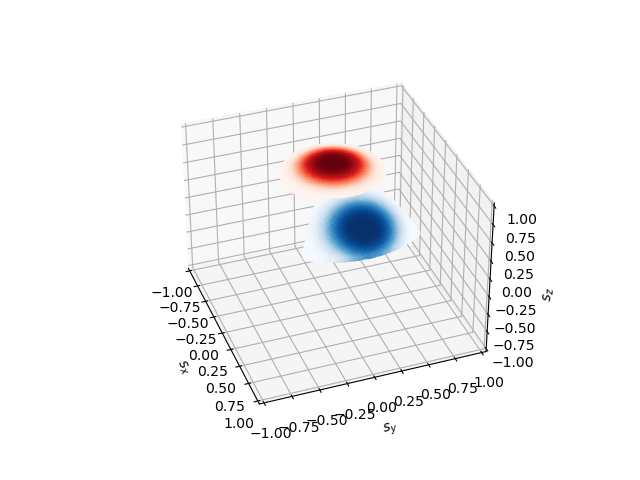
\includegraphics[width=\textwidth]{fig3a.png}
	\end{subfigure}
	\begin{subfigure}{0.74\textwidth}
		\subcaption{}
		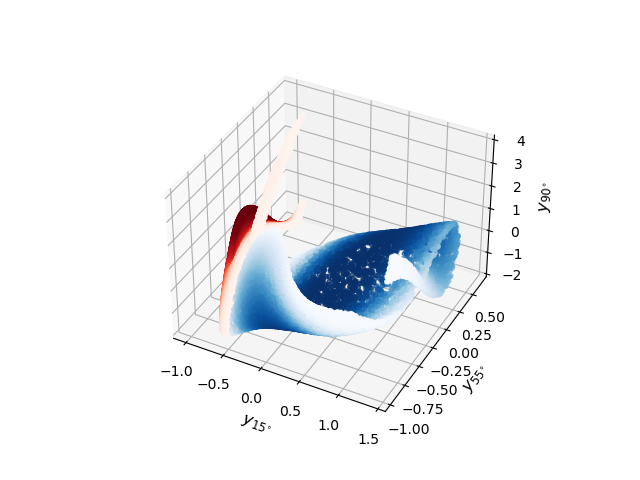
\includegraphics[width=\textwidth]{fig3b.png}
	\end{subfigure}
	\caption{(a) Distribution of orientation vectors and (b) their respective scattering signals. Points are coloured according to their distance from the centre of each cluster (red points centred around [$0.00, 0.00, 1.00$], blue points centred at [$0.71, 0.00, 0.71$])}
	\label{fig:mixing}
\end{figure}

Nevertheless, at least where the uncertainty in signal measurements 
is low, we can predict the orientation from the scattering scattering 
by utilising computational techniques such as neural networks. We 
thus utilised the Python machine learning program \textit{scikit-learn} \cite{Pedregosa2011} to build a neural network for identifying the 
dimer's orientation from its light scattering signal. The network 
was trained by generating a database of random orientation vectors, 
calculating the corresponding light scattering signals, and then 
using the network to estimate the probability of a given signal coming 
from a dimer in a given reference orientation. The network's loss 
function was evaluated and used to improve the estimation, the 
network being trained until the improvement in the loss function 
was less than 0.0001. 

Importantly, the estimation provided by the neural network can be 
improved further by accounting for any prior information we know 
about the dimer, utilising Bayesian inference to update the neural 
network's estimation: 
\begin{align}
	\label{eq:bayes}
	p(\hat{\bf n}_\alpha| y_k(\hat{\bf s}))
	&=
	\frac{p(y_k(\hat{\bf s})|\hat{\bf n}_\alpha)
		p(\hat{\bf n}_\alpha)}{p(y_k(\hat{\bf s}))}
\end{align}

where $p(\hat{\bf n}_\alpha)$ and $p(y_k(\hat{\bf s}))$ are the prior 
estimates of the distributions of particle orientations and 
instantaneous signals, respectively. \textit{Without} any prior 
evidence we must assume that the orientation prior of the dimer 
$p(\hat{\bf n}_{\alpha})$ is uniform. However, inference about the 
dimer's possible current orientation from knowledge of previous 
measurements can be used to inform our estimate of $p(\hat{\bf 
n}_{\alpha})$. The latter prior $p(y_k(\hat{s}))$ is the probability of 
measuring a signal ($y_1$, $y_2$, $y_3$). This is given by taking 
the discrete integral over the collection of reference orientations:
\begin{align}
	p(y_k(\hat{\bf s}))
	=
	\sum_{\alpha=1}^{n_{\rm ref}}
	p(y_1, y_2, y_3, y_4|\hat{\bf n}_\alpha)
	p(\hat{\bf n}_\alpha)
\end{align}

From \eqref{eq:bayes} we obtain the key result, a mass probability 
distribution denoting the probability that our dimer is in 
orientation $\hat{\bf n}_{\alpha}$ given a measured signal ($y_1$, 
$y_2$, $y_3$), \textit{i.e.} an estimated mapping from scattering 
measurement to orientation estimate. 

%%%%%%%%%%%%%%%%%%%%%%%%%%%%%%%%%%%%%%%%%%%%%%%%%%%%%%%%%%%%%%%%%%%%%
\subsection{Calculation of error}
\label{sec:divergence}
Using \eqref{eq:bayes} we get a snapshot estimation of the instantaneous
orientation of the trapped dimer based on a single measurement from a 
collection of detector signals. Of course in reality these detectors 
will be returning a discrete time series representative of the dimer's
trajectory within the optical trap. 

Using the simulation code from \cite{Vigilante2020} we can replicate 
this trajectory and furthermore use \textit{mstm}to calculate the far field 
intensity produced by said dimer. At each time step we measure the signal
produced at each measurement angle and use our neural network to calculate
$p(y_k(\hat{\bf s})|\hat{\bf n}_\alpha, t)$. 

Evaluating how well Eq.~\eqref{eq:bayes} performs in predicting $\hat{\bf n}$
is difficult because we have discretised the orientation space meaning 
there will always be some degree of inaccuracy in our prediction. The Kullback-Liebler divergence method provides a measure of the relative
entropy change between two probability distributions:
\begin{align}
	D_{KL}(P(t)\parallel Q(t)) = \sum P(t) \log_2\left[\frac{P(t)}{Q(t)}\right] 
	\label{eq:D_KL}
\end{align} 

Where $P(t)$ and $Q(t)$ are two probability distributions we are
comparing, often it is common to use a base 2 log as this converts 
the entropy to base 2. By relative entropy we are talking about 
the useful information gained/lost by switching from $P(t)$ to 
$Q(t)$. In our case $Q(t)$ is simply the distribution given by
Eq.~\eqref{eq:bayes} and $P(t)$ is an idealised distribution, 
one where the model is accurate with 100\% certainty.
\begin{align}
	\label{eq:best}
	p_{best} = P(t) =
	\begin{cases}
		1 & \text{when $\hat{\bf n}_\alpha$ = $\hat{\bf n}_{best}$}\\
		0 & \text{when $\hat{\bf n}_\alpha$ $\neq$ $\hat{\bf n}_{best}$}
	\end{cases}
\end{align}

In reality the distribution from Eq.~\eqref{eq:bayes} will assign 
some non-zero probability to every reference orientation. Therefore 
the relative entropy for a single measurement is given as:
\begin{align}
	D_{KL}(p_{best}\parallel p(\hat{\bf n}_\alpha| y_k(\hat{\bf s}), t))
	= \log_2 \left[\frac{1}{p(\hat{\bf n}_\alpha| y_k(\hat{\bf s}), t)}
	\right]
	\label{eq:kullback}
\end{align}

The relative entropy is a measure if how spread out our distribution
is. With larger values of $D_{KL}$ indicating that our prediction is 
spread out so the neural net is unsure about $\hat{\bf n}_{best}$. 
Whereas a low value of $D_{KL}$ means that our model is more confident 
in $\hat{\bf n}_{best}$. The only draw back being that the relative 
entropy does nothing to indicate accuracy, only how closely our 
distribution matches our ideal result. This will be better 
exemplified later in \ref{sec:test}.
%%%%%%%%%%%%%%%%%%%%%%%%%%%%%%%%%%%%%%%%%%%%%%%%%%%%%%%%%%%%%%%%%%%%%
%%%%%%%%%%%%%%%%%%%%%%%%%%%%%%%%%%%%%%%%%%%%%%%%%%%%%%%%%%%%%%%%%%%%%
\subsection{Brownian Simulation}
\label{sec:brownian}

We use the Brownian OT package developed by Fung~\textit{et~al} 
\cite{Vigilante2020} to simulate the motion of an asymmetric dimer (Figure~\ref{fig:dimer}a) within an optical trap. We simulate the 
motion of a dimer trapped in a highly focused Gaussian beam by 
calculating the optical forces imparted by the laser, and the 
Brownian force due to the surrounding fluid. We simulated a 
polystyrene dimer ($n = 1.59$) in a suspension of water ($n_{med} 
= 1.33$). As discussed in chapter 4 dimers can be stably trapped
in off-axis orientations. We simulate a dimer (of size ratio 2) that
is trapped in this off-axis orientation by a $5 mW$ laser, due to 
the meta-stability of the trap the dimer is only trapped for second
before it escapes the trap. The dimer's position and orientation 
is shown below:
\begin{figure}[h!]
	\centering
	\begin{subfigure}{0.45\textwidth}
		\subcaption{}
		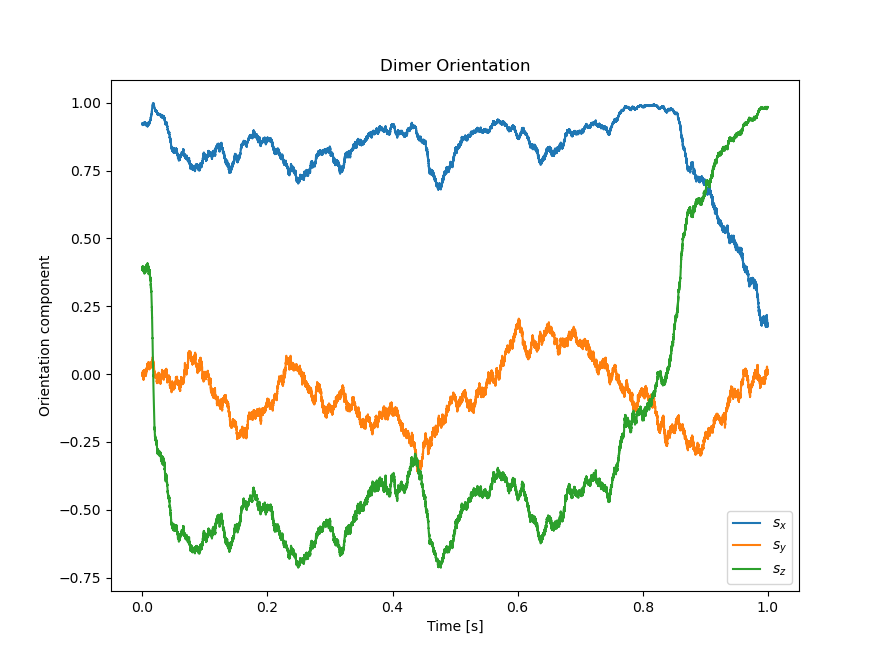
\includegraphics[width =\textwidth]{fig7a.png}
	\end{subfigure}
	\begin{subfigure}{0.45\textwidth}
		\subcaption{}
		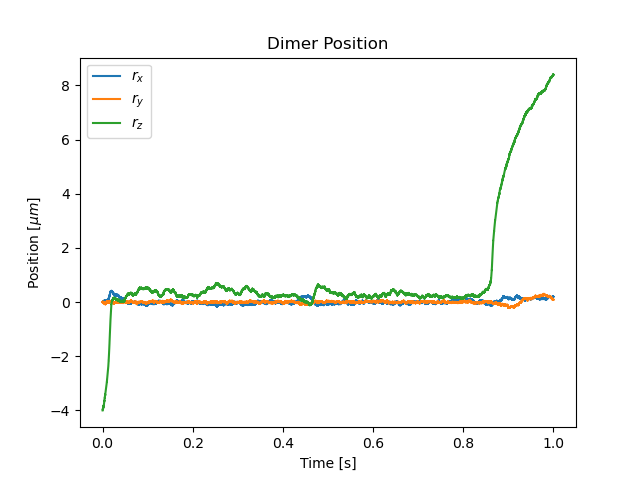
\includegraphics[width=\textwidth]{fig7b.png}
	\end{subfigure}
	\caption{Simulation results of: (a) the dimer's orientation vector with time, (b) the dimer's [x,y,z] position with time.}
	\label{fig:motion}
\end{figure}

At the same we use \textit{mstm} to replicate the intensity of light
incident on the surfaces of detectors placed around the focus of the
optical trap. The exact number of detectors was initially assumed to 
be arbitrary, in that it made no difference to our estimate whether 
we used 2 angles or 200.

\subsection{Choice on the number of detectors}
When all of the detectors lie in the same plane the expected signal 
can appear identical despite the dimer being in completely different orientations. It should be noted that these pairs are reflected in 
one or more axis which suggests that these are due to the arrangement 
of our detectors. More specifically, if the detectors are placed say 
in the x-y plane then only when the dimer is pointed nearly fully 
upright will the expected signal be entirely unique. This is not an 
issue with typical analytical static light scattering experiments 
because the signal being collected is averaged over a population of 
particles all in different orientations. Whereas in our set up we are concerned with the scattering of a single particle whose scattering is orientationally dependant. 

To remedy this we raise the third detector out of the x-y plane; 
as such the expected signals from each reference orientation is 
unique, though with limited resolution. By adding a $4^{th}$ 
detector we can differentiate signals more reliably, improving the 
neural networks performance. In line with our goal of making this 
method viable in a laboratory setting we decided not to increase 
the number of detectors further than 4. 

%%%%%%%%%%%%%%%%%%%%%%%%%%%%%%%%%%%%%%%%%%%%%%%%%%%%%%%%%%%%%%%%%%%%%
\section{Testing the Neural Network}
\label{sec:test}
We applied Eq.~\eqref{eq:bayes}, taking the reference orientation 
with the highest probability  as our estimate of the dimer's 
instantaneous orientation $\hat{\bf n}_{est}$. To visualise the 
model's performance we plotted the orientation components of our 
estimation $\hat{\bf n}_{\alpha}$ and the dimer's \emph{actual} 
instantaneous orientation $\hat{\bf s}$ versus time. For comparison, 
we also plotted the orientation components of the closest reference orientation, $\hat{\bf n}_{best}$. Assuming a uniform prior of the 
reference orientations $p(\hat{\bf n}_\alpha)$ the neural network's predictions ($\hat{\bf n}_{\alpha}$ from Eq.~\eqref{eq:bayes}) are 
at times reasonable, but there are significant large and random jumps 
away from the correct result (Fig.~\ref{fig:uniform}). 
\begin{figure}[h!]
	\centering
	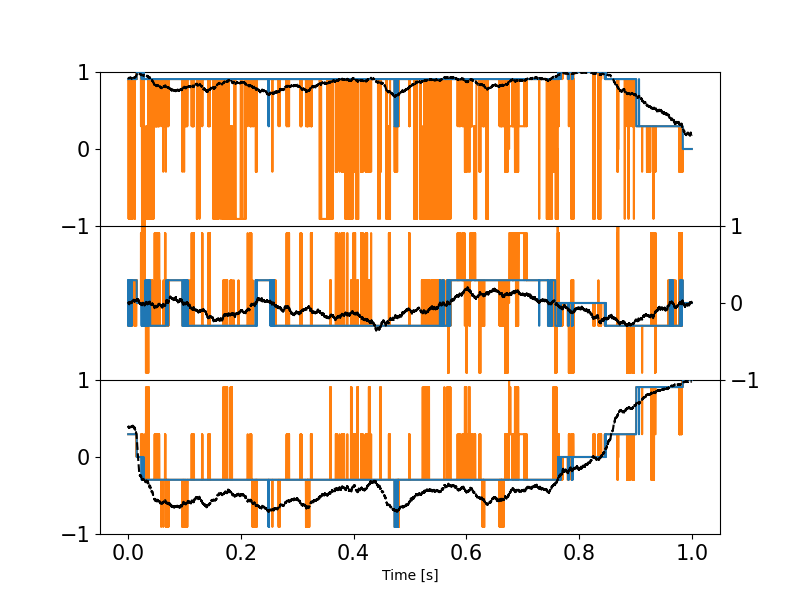
\includegraphics[width=\textwidth]{fig5.png}
	\caption{Model's estimation of dimer orientation over the simulation time, assuming uniform prior $p(\hat{\bf n}_\alpha)$, broken up into x, y, and z components for clarity. Blue line denotes the best result we can achieve (the reference orientation $\hat{\bf n}_{best}$ that is closest to the actual orientation), orange line denotes the result provided by eq~\ref{eq:bayes}: where the blue line is not visible, the model's prediction agrees with $\hat{\bf n}_{best}$. Dotted black line is the instantaneous orientation $\hat{\bf s}$.}
	\label{fig:uniform}
\end{figure} 

One reason we observe such large jumps in the estimated 
orientation is simply because the neural network is assuming
that the signals are unrelated from one another. We can 
observe this if we take the average relative entropy change
across the entire trajectory:

\begin{align}
	\langle D_{KL}\rangle = \frac{1}{N} \sum_{i=1}^{N} \log_2 \left[\frac{1}{p(\hat{\bf n}_\alpha\parallel y_k(\hat{s}),t_i)}\right]
	\label{eq:score}
\end{align}

Where we get an average entropy change of $\approx 0.604$, in 
base 2 this means that on average the model has narrowed down 
its options from 1 in 30 to 1 in 1.52. This is not reflected
though in fig.~\ref{fig:uniform} which indicates that while 
the model is highly confident in its results it is not at all 
accurate. As demonstrated by fig~\ref{fig:mixing} the 
orientation and signal spaces are uncorrelated with one another 
which results in the neural network to assign orientations 
incorrectly. Combining this fact with use of a uniform prior 
($p(\hat{\bf n}_\alpha)$), there is no constraint on how much 
estimated orientation can change from time-step to time-step. 

To improve the estimation we can therefore use knowledge of the 
physical limitations of the object in the trap and its dynamics. 
Imposing a more physically grounded prior, accounting in this case 
for the fact that the rotational motion of the dimer is limited by 
the rotational trap stiffness ($\kappa_r$). Here the prior of the 
reference orientations $p(\hat{\bf n}_\alpha)$ was redefined at 
each time step as a Boltzmann distribution of the physical distance 
between the previous estimate $\hat{\bf n}_{est}(t-\Delta t)$ and 
each reference orientation $\hat{\bf n}_\alpha$. Put simply, we are 
reweighing our estimation based on the size of rotation, with smaller movements being favoured over large movements:
\begin{align}
	p(\hat{\bf n}_\alpha)
	&=\frac{e^{\hat{\bf n}_\alpha 
			\cdot \hat{\bf n}_{est}(t-\Delta t)}}
	{\sum_{\alpha=1}^{n_{\rm ref}}
		e^{\hat{\bf n}_\alpha 
			\cdot \hat{\bf n}_{est}(t-\Delta t)}}
	\label{eq:boltz}
\end{align}

As shown in Figure~\ref{fig:biased} implementation of Eq~\eqref{eq:boltz} helps significantly reduce the large random excursions of estimated orientation away from the 'best' result. However at the same 
time result is still subpar.
\begin{figure}[h]
	\centering
	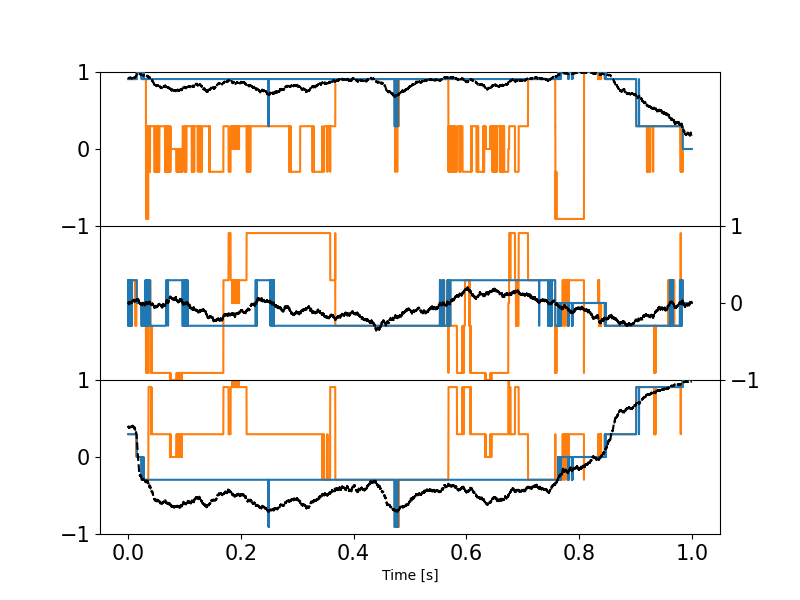
\includegraphics[width=\textwidth]{fig8a.png}
	\caption{\label{fig:biased}
		%
		Estimation of dimer orientation with $p(\hat{\bf n}_\alpha)$ defined
		by Eq~\eqref{eq:boltz}.  Blue line denotes the best result we can
		achieve, orange line denotes the result provided by eq~\ref{eq:bayes}.
		Dotted black line is the instantaneous orientation $\hat{\bf s}$ (see Section~\ref{sec:Bayes}).
		%
	}
\end{figure} 

Once again using Eq.~\eqref{eq:score} we now get a result of 
$\approx 0.204$ or a 1 in 1.2 result. This is only a slight 
improvement in terms of confidence but has drastically reduced 
the variation in our models predictions. There are other 
improvements that can be made, which additionally also help with
potential sources of error in our set up.

%%%%%%%%%%%%%%%%%%%%%%%%%%%%%%%%%%%%%%%%%%%%%%%%%%%%%%%%%%%%%%%%%%%%%
%%%%%%%%%%%%%%%%%%%%%%%%%%%%%%%%%%%%%%%%%%%%%%%%%%%%%%%%%%%%%%%%%%%%%
\section{Accounting for sources of error in light scattering measurements}
When it comes to analysing light scattering from any size particle,
error analysis becomes a significant factor. Typically this can be 
accounted for by averaging over long periods of time to get an 
assessment of the steady state conditions of the target particle. 
However in our case where we wish to know the instantaneous 
orientation, we instead have to rely on our understanding of how 
uncertainty can effect our model's performance. We identified two 
areas which are likely sources of error in our estimation: firstly, 
an incorrect modelling of the target particle, and secondly, signal 
noise arising from experimental factors. We highlight how we address 
these areas below. 
%%%%%%%%%%%%%%%%%%%%%%%%%%%%%%%%%%%%%%%%%%%%%%%%%%%%%%%%%%%%%%%%%%%%%
\subsection{Impact of incorrect dimer sizing}
\label{sec:lam}

One of the main limitations of our model is that we assume that 
the dimer being modelled in \textit{mstm} is accurate to the 
dimer being trapped in the optical tweezer. Sizing molecules 
accurately is a significant challenge for single particle 
analysis so there is bound to be some uncertainty with the 
measurements. We ran our model 3 times with the neural net being 
trained on a dimer of size ratio $1:1.95$, $1:2.00$ and $1:2.05$.
\begin{figure}[h!]
	\centering
	\begin{subfigure}{0.33\textwidth}
		\subcaption{}
		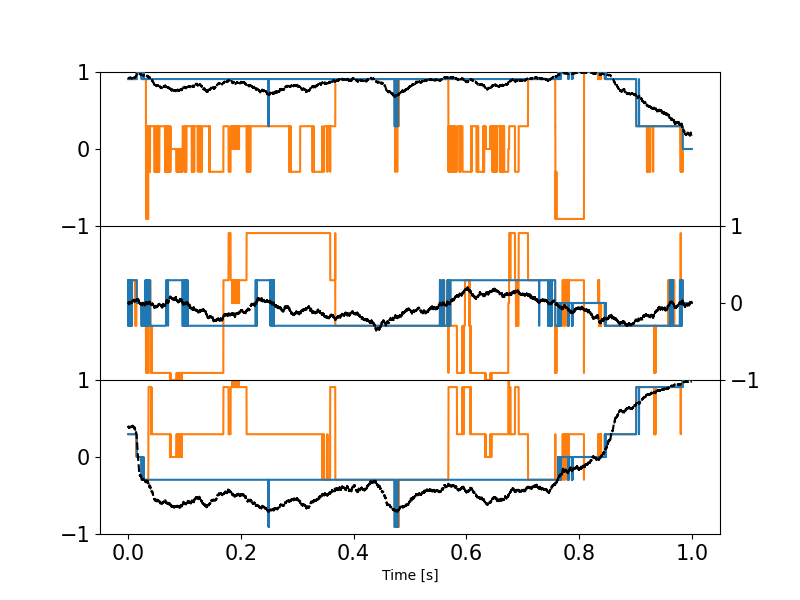
\includegraphics[width =\textwidth]{fig8a.png}
	\end{subfigure}
	\begin{subfigure}{0.31\textwidth}
		\subcaption{}
		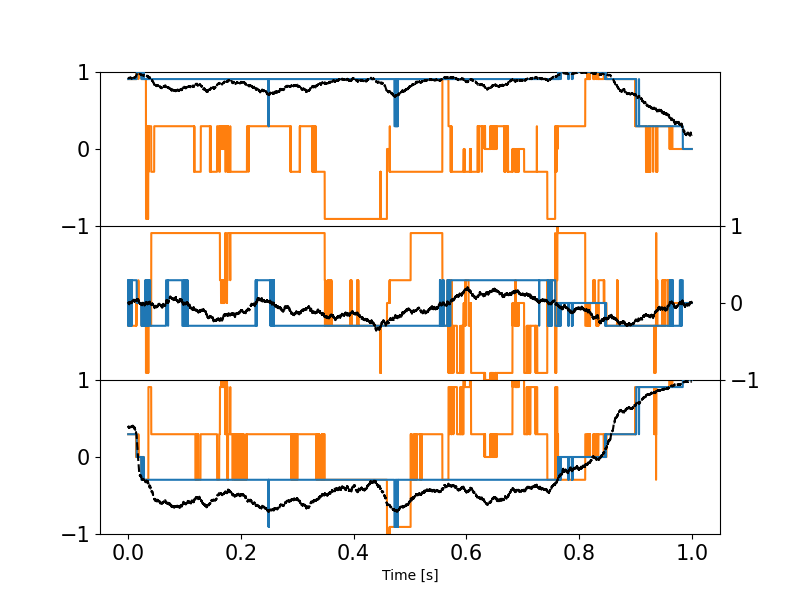
\includegraphics[width=\textwidth]{fig8b.png}
	\end{subfigure}
	\begin{subfigure}{0.31\textwidth}
		\subcaption{}
		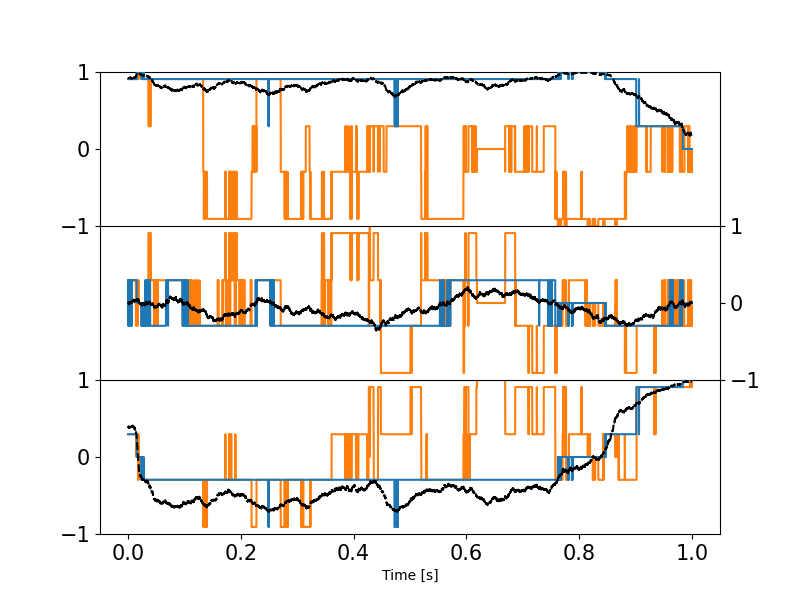
\includegraphics[width=\textwidth]{fig8c.png}
	\end{subfigure}
	\caption{Model estimates of orientation when neural net has 
		been trained on dimer of size ratio: (a) 1:2 $[\langle D_{KL}\rangle=0.519]$, (b) 1:2.05 $[\langle D_{KL}
		\rangle=3.706]$, (c) 1:1.95 $[\langle D_{KL}\rangle=
		3.705]$ ($n_{refs} = 30$)}
	\label{fig:size}
\end{figure}

As can be seen from Fig~\ref{fig:size}  even the slightest change in size ratio makes a very significant difference to the performance of our model. This amounts to just over $100 \ nm$ in the dimer's overall size, yet results in our model being correct from over 90 \% of the time to now as low as 30 \%. This highlights the importance of correctly sizing trapped entities before performing any in depth analysis of the scattering pattern, as even the slightest deviation can have a serious impact. We addressed this by increasing the number of available reference orientations from 30 to 126 (following the same procedure as given by \cite{Reyuthor2006} to evenly space out the coordinates) and increasing the weighting factor in Eq~\ref{eq:boltz}. While this didn't have a significant improvement on the overall accuracy of the model, in the worst case having a slight increase from 30.5 \% to 40.3 \%, it did help to significantly reduce the magnitude between our model's estimations and the dimer's motion as seen below in Fig~\ref{fig:refs}.
\begin{figure}[h!]
	\centering
	\begin{subfigure}{0.31\textwidth}
		\subcaption{}
		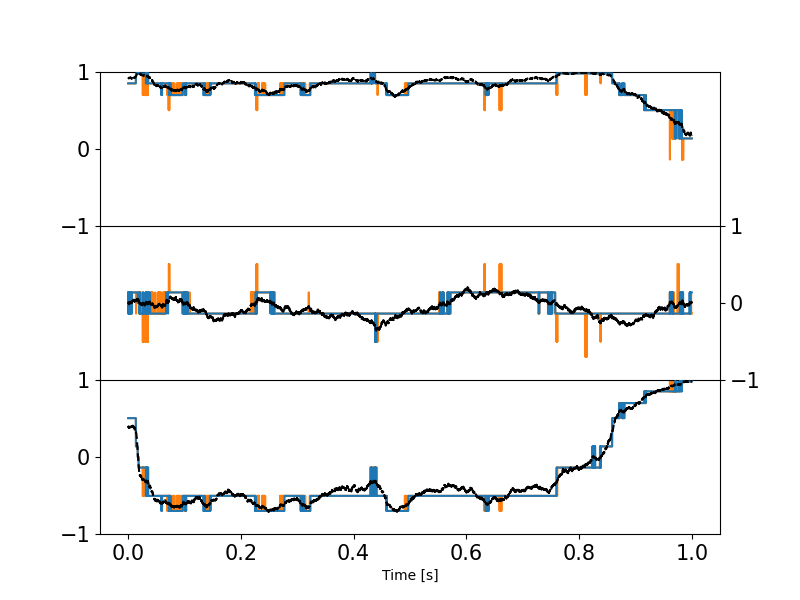
\includegraphics[width =\textwidth]{fig9a.png}
	\end{subfigure}
	\begin{subfigure}{0.31\textwidth}
		\subcaption{}
		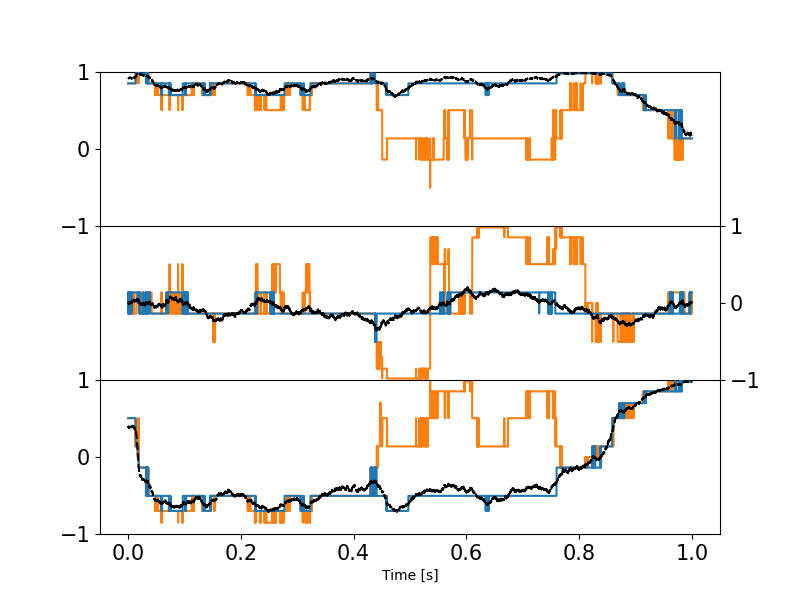
\includegraphics[width=\textwidth]{fig9b.png}
	\end{subfigure}
	\begin{subfigure}{0.31\textwidth}
		\subcaption{}
		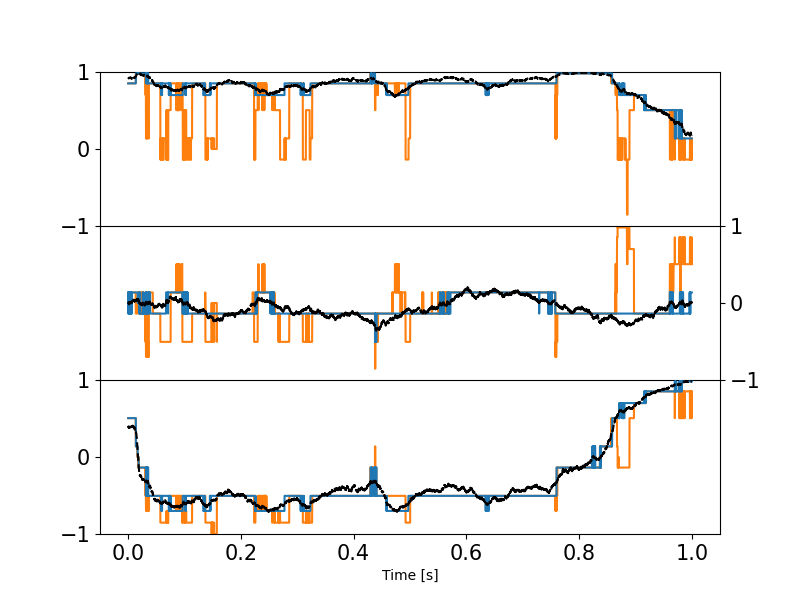
\includegraphics[width=\textwidth]{fig9c.png}
	\end{subfigure}
	\caption{Model estimates of orientation when neural net has 
		been trained on dimer of size ratio: (a) 1:2 $[\langle D_{KL}\rangle=0.593]$, (b) 1:2.05 $[\langle D_{KL}\rangle
		=5.659]$, (c) 1:1.95 $[\langle D_{KL}\rangle=3.279]$, 
		($n_{refs} = 126$)}
	\label{fig:refs}
\end{figure}

Notably the increasing the number of reference orientations had a greater effect when our neural network was trained on a 1:1.95 dimer than a 1:2.05 dimer. This suggests that overshooting our size estimate will be less detrimental to our estimation. Notably if the our sizing is off the neural network does not predict a smooth motion within the trap; instead predicting that the dimer is jumping back and forth between different orientations. This suggest that we can narrow down our estimate of the particle's size by assessing how the dimer is reorienting within the trap, as we should expect a smooth continuos prediction. Since we are working with a spherical dimer it also stands to reason that techniques such as image analysis could be used in part to address this, so long as the trapped entity is sufficiently illuminated. 
%%%%%%%%%%%%%%%%%%%%%%%%%%%%%%%%%%%%%%%%%%%%%%%%%%%%%%%%%%%%%%%%%%%%%
\subsection{Impact of measurement noise on model predictions}
\label{sec:epsilon}

So far a key assumption of the neural network implementation is that the detected scattering signal has no uncertainty associated with it. In reality of course scattering signals will always have some non-zero measurement noise. This can be attributed to a variety of factors, from a measurement bias in the detector, to the Brownian motion of the dimer itself. To explore the impact of measurement uncertainty on orientation estimation model performance we introduce a Gaussian noise to the measured signal:
\begin{align}
	I(\hat{\bf s}) = I(\hat{\bf s}) \pm \epsilon I(\hat{\bf s})
\end{align}
where $\epsilon$ is the percentage error associated with the scattering signal. Figure~\ref{fig:epsilon} shows the performance of the model at a range of $\epsilon$ using in-plane detector angles $15^{\circ}$, $55^{\circ}$, $90^{\circ}$ and out-of-plane detector at $75^{\circ}$, with $\beta$ set to $1$:

\begin{figure}[h!]
	\centering
	\begin{subfigure}{0.32\textwidth}
		\subcaption{}
		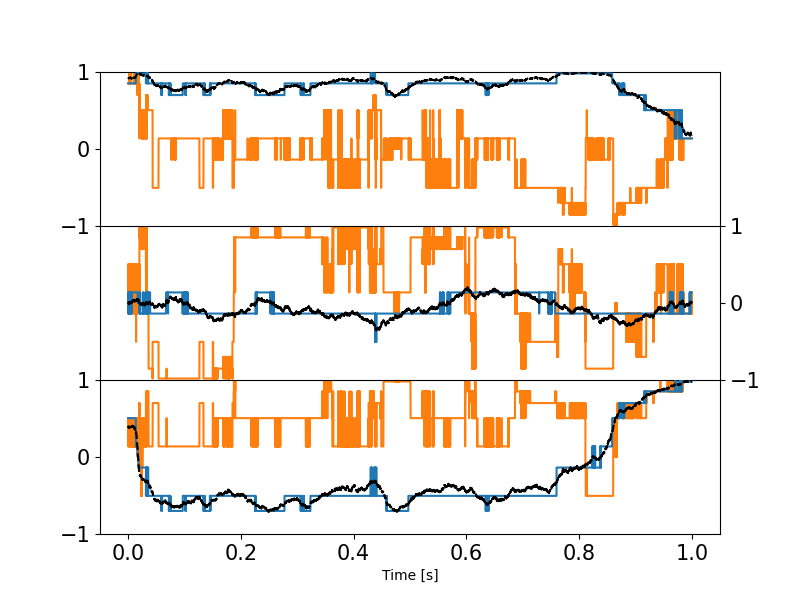
\includegraphics[width=\textwidth]{fig10a.png}
	\end{subfigure}
	\begin{subfigure}{0.32\textwidth}
		\subcaption{}
		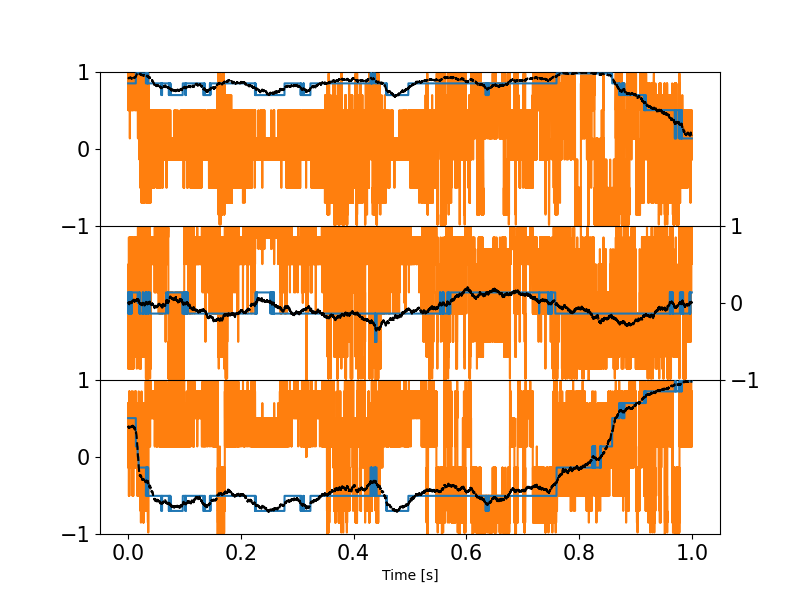
\includegraphics[width=\textwidth]{fig10b.png}
	\end{subfigure}
	\begin{subfigure}{0.32\textwidth}
		\subcaption{}
		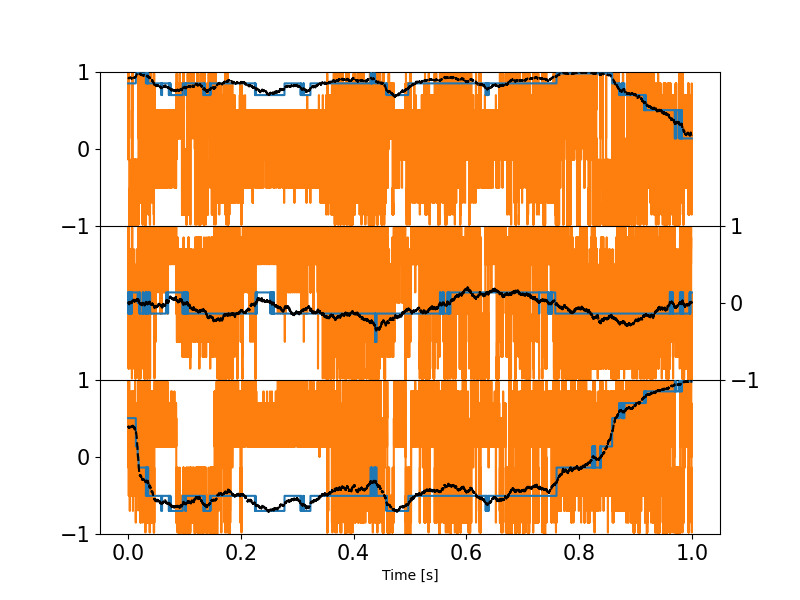
\includegraphics[width=\textwidth]{fig10c.png}
	\end{subfigure}
	\caption{Model prediction for signal error of (a) $1\%$ ~
		$[\langle D_{KL}\rangle=0.962]$, (b) $15\%$ $[\langle D_{KL}\rangle=13.654]$, and (c) $25\%$ ~  $[\langle D_{KL}\rangle=13.017]$.}
	\label{fig:epsilon}
\end{figure}

As can be seen from Figure~\ref{fig:epsilon}, the inclusion of 
signal noise quickly leads to a decrease in the model's 
performance. So much so that beyond 15\% the model is actually 
worse than just randomly guessing.This is due to an inherent 
feature of the inverse scattering problem: two distinct regions 
in orientation space can become heavily intertwined and thus no 
longer well separated when mapped to intensity space (even 
though the mapping remains continuous): so even small 
uncertainties in the scattering data can lead to large 'mistakes' 
in the choice of orientation by the neural network. (Indeed if 
this was not the case the inverse scattering problem would be 
quite simple.) 

To reduce the effects of the signal noise we took the time 
average of the expected signal over $0.001 s$ and then had our 
neural network estimate the orientation based on the average 
signal.

\begin{figure}[h!]
	\centering
	\begin{subfigure}{0.32\textwidth}
		\subcaption{}
		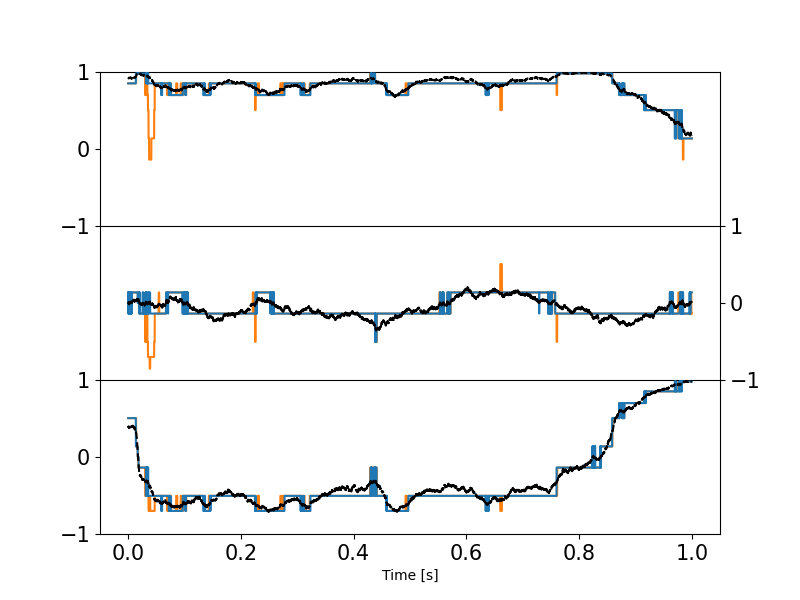
\includegraphics[width=\textwidth]{fig11a.png}
	\end{subfigure}
	\begin{subfigure}{0.32\textwidth}
		\subcaption{}
		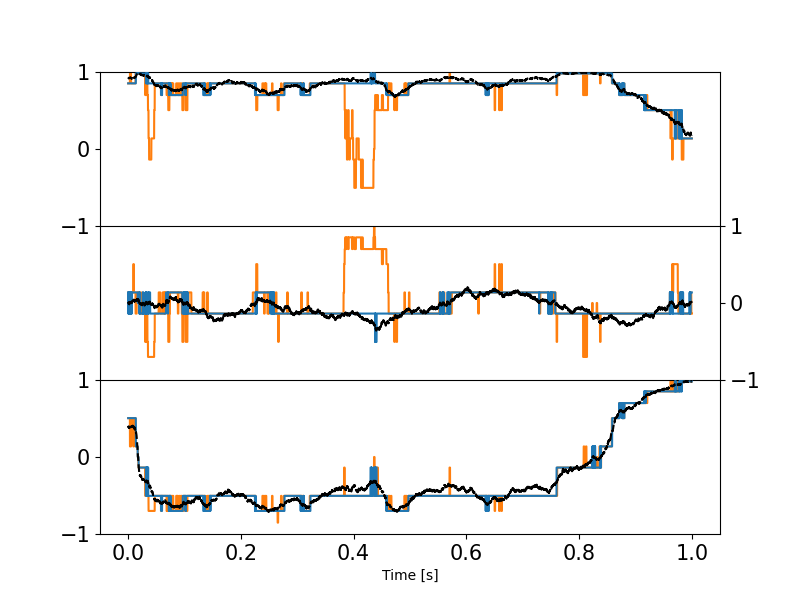
\includegraphics[width=\textwidth]{fig11b.png}
	\end{subfigure}
	\begin{subfigure}{0.32\textwidth}
		\subcaption{}
		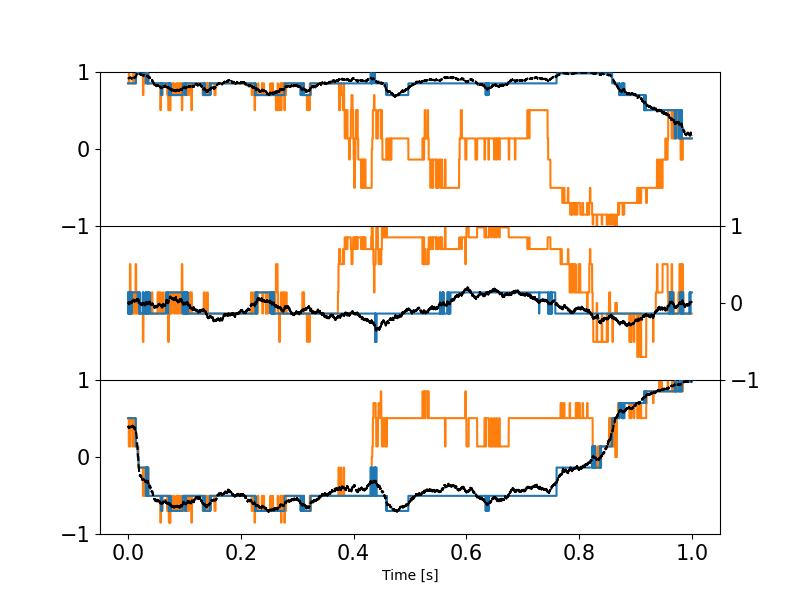
\includegraphics[width=\textwidth]{fig11c.png}
	\end{subfigure}
	\caption{Model prediction for signal error of (a) $1\%$ 
		$[\langle D_{KL}\rangle=1.447]$, (b) $15\%$ $[\langle D_{KL}\rangle=4.670]$, and (c) $25\%$ $[\langle D_{KL}
		\rangle=7.911]$, time averaged over $1\,{\rm ms}$}
	\label{fig:time average}
\end{figure}
This resulted in a reduction in the overall signal noise and 
provided a higher degree of accuracy for our model. There 
appears to be no clear correlation between the length over 
which we time average and the performance of our model. Time 
averaging over every 0.05s resulted in a drastically worse 
performance; this is due to the fact that over longer time 
periods there is greater uncertainty regarding how the dimer's 
orientation has changed, thus tracking the instantaneous 
orientation becomes harder for the neural network. Fortunately, 
time averaging even over $1\,{\rm ms}$ seems to provide a 
satisfactory estimation of the dimer's angular dynamics within 
the optical trap.

Overall it’s clear that estimation of the dimer’s orientation 
is a problem that can be endlessly tuned to optimise the 
result. Here we simplify the problem somewhat by employing 
a relatively small finite number of 'reference orientations' 
to map between scattering and dimer orientation: the precision 
of estimation could be improved by utilising a greater number 
of reference orientations, although there remains a balance 
between the realisable precision of orientation estimate and 
the noise level of the scattering measurement. 
Another avenue to further explore would be using 
the method to optimise the choice of detection angles, 
essentially to find the region in the mapping between measured 
scattering and orientation that others the best degree of 
confidence through optimal separation of scattering signals 
for distinct orientations. For sequences of data such as 
dynamic measurements, a further potential enhancement would 
be to consider more complex correlations based on prior 
expectations of the dynamics. The Debye equation for  Here already we improve the 
method using a non-uniform prior based on only the immediately 
previous measurement in time (see Section 2.1): considering 
a non-uniform grouping of reference orientations might result 
in a better estimation, if we have information regarding the 
dimer’s preferred axis of rotation. 

%%%%%%%%%%%%%%%%%%%%%%%%%%%%%%%%%%%%%%%%%%%%%%%%%%%%%%%%%%%%%%%%%%%%%
\section{Conclusion}
\label{sec:Conclusion}

We have developed a method for measuring the dynamics of an 
optically-trapped colloidal objects based purely on 
measurements of the object's light scattering at a small 
number of detection angles. We demonstrate the method using 
the orientation of an asymmetric dimer as the dynamic variable 
and object of interest respectively, but in principle the 
model can be applied to any characteristic that impacts the 
light scattering pattern produced by a trapped entity such 
as size and shape. The MSTM package is a flexible tool for 
calculating the light scattering of complex objects using a 
representation of the object as a set of micro-particles, 
enabling training of a neural network to enable categorisation 
of the mapping between scattering and trapped object 
characteristics. By taking account of the physically realistic 
behaviour of the trapped object and the characteristics of 
the trap (which impact the dynamics of the object), the 
Bayesian inference method can be re ned to provide a reliable 
estimation of object characteristics of interest, even in the 
presence of measurement noise. Fundamentally, the inverse 
scattering problem is difficult to solve, since the mapping 
between object characteristics and scattering can be highly 
complex. We determined the minimum number of detectors 
required for a reliable estimation in the presence of 
measurement noise; furthermore, we demonstrated that the 
arrangement of these detectors is critical for a reliable 
estimation of an objects orientation. However, Bayesian 
inference based on neural network estimation of the mapping 
provides a powerful method for practical applications, 
extending the use of optical trapping beyond measuring 
microscopic force response toward detailed structural and 
dynamic information about complex trapped entities. 

Conventional calibration methods will not be adequate however, while
angular motion can be detected using complicated set ups \cite{Bang2020},
this can only provide an estimate of the magnitude of a particle's 
angular motion. This is perfectly fine in cases where the rotational
motion is stochastic and intuitively predictable (i.e. a dimer in a
vertical orientation undergoing stochastic Brownian motion), but in 
the case the the motion is instead periodic characterising it requires
instantaneous measurements of the particle's motion. 

